% ============================================================
%  Fault-Tolerant Multimodal Presence Verification
%  CPRE 5450: Dependable Computing Systems -- Shobhit Singh
%  Iowa State University, Spring 2026
%
%  BUILD WITH MiKTeX (command line):
%    pdflatex Singh_Shobhit_CPRE5450_Report.tex
%    pdflatex Singh_Shobhit_CPRE5450_Report.tex   (2nd pass for TOC/refs)
%
%  Or: MiKTeX Console -> Tasks -> Build -> Process file
%  Packages auto-install on first compile if "Install on-the-fly" is ON.
% ============================================================

\documentclass[12pt]{extarticle}
\usepackage[left=1in,right=1in,top=1in,bottom=1in]{geometry}
\usepackage[title,toc]{appendix}
\usepackage{amsmath}
\usepackage{booktabs}
\usepackage{gensymb}
\usepackage{graphicx}
\usepackage[colorlinks=true,linkcolor=black,citecolor=black,urlcolor=blue]{hyperref}
\usepackage{listings}
\usepackage{microtype}
\usepackage{setspace}
\usepackage{titlesec}
\usepackage{times}
\usepackage{float}
\usepackage{tikz}
\usepackage{xcolor}
\usepackage{array}
\usepackage{tabularx}
\usetikzlibrary{arrows.meta,positioning,shapes,fit,calc,automata}

\lstset{
  basicstyle=\footnotesize\ttfamily,
  columns=fullflexible,
  frame=single,
  breaklines=true,
  keywordstyle=\color{blue}\bfseries,
  commentstyle=\color{gray},
  stringstyle=\color{orange!70!black},
  numbers=left,
  numberstyle=\tiny\color{gray},
  numbersep=5pt,
  tabsize=4
}

\title{\textbf{Fault-Tolerant Multimodal Presence Verification}\\[6pt]
       \textbf{and Safe Activation Policies on ESP32-S3}\\[6pt]
       \textbf{Using mmWave Radar and Vision}}
\author{Shobhit Singh\\[10pt]
        \normalsize Department of Electrical and Computer Engineering\\
        Iowa State University}
\date{May 11, 2026}

\begin{document}
\maketitle
\thispagestyle{empty}
\vfill
{\centering \LARGE
  Project Report\\
  CPRE~5450: Dependable Computing Systems\\[12pt]
  Iowa State University\\
  Spring 2026
\par}
\vspace*{0.8in}

\clearpage
\subsection*{\centering \normalfont ABSTRACT}
{\large
Assistive room-scale embedded systems increasingly rely on edge perception to decide when to
activate high-power sensing and interaction (camera inference, audio capture, actuation).
However, these systems face frequent faults and uncertainties including lighting-induced
vision degradation, radar clutter, transient communication errors, timing variability, and
resource constraints.
A single-modality activation scheme is therefore brittle and can produce two critical
failure modes: (i)~false activations that waste energy and may raise privacy concerns,
and (ii)~missed activations that deny assistance and reduce system trustworthiness.

This project proposes a fault-tolerant activation subsystem implemented on an ESP32-S3
platform integrating a camera module and a 24~GHz FMCW mmWave radar module.
The approach uses heterogeneous redundancy and system-level diagnosis: mmWave provides
presence cues robust to lighting and can be privacy-preserving, while vision provides
spatial confirmation and helps resolve radar ambiguities.
The subsystem performs cross-sensor consistency checks and temporal redundancy to detect
inconsistencies, classifies them into transient versus persistent faults, and selects
recovery actions accordingly.

A two-tier safe-state policy is introduced.
In a \emph{soft safe state}, the system suppresses full activation and performs
re-validation under a bounded time window; in a \emph{hard safe state} (persistent
inconsistency), the system blocks activation, isolates low-confidence inputs, and
optionally provides user feedback while maintaining minimal power consumption.
Design choices are guided by multi-source sensor fusion research that explicitly
addresses cross-sensor inconsistency and uncertainty quantification, and by radar
presence-detection research that motivates OOD-aware monitoring for cluttered indoor
environments.

Evaluation will combine controlled fault injection (sensor packet drops, radar framing
errors, camera frame corruption/blur, induced timing delays) with environmental stress
tests (low light, reflective surfaces, moving clutter).
Metrics include false activation rate, missed activation rate, time-to-detect
inconsistency, fault coverage, and activation latency/energy overhead relative to a
non-fault-tolerant baseline.

This work demonstrates how classical fault-tolerance principles---redundancy, error
detection, diagnosis, and graceful degradation---can be concretely applied to practical
edge AI activation pipelines on resource-constrained embedded hardware, improving
reliability and trustworthiness for assistive room settings.
}

\clearpage
\tableofcontents

\clearpage
\titlespacing\section{0pt}{14pt plus 4pt minus 2pt}{4pt plus 2pt minus 2pt}
\titlespacing\subsection{0pt}{10pt plus 2pt minus 2pt}{2pt plus 1pt minus 1pt}
\titlespacing\subsubsection{0pt}{8pt}{2pt}
\setlength{\parskip}{0.45\baselineskip}
\setlength{\parindent}{0pt}

%=================================================================
\section{Introduction}
\label{sec:intro}

\subsection{Motivation}

Room-scale assistive systems must decide when to wake up, when to sense, and when to
interact.
This decision is especially critical in privacy-preserving systems for blind or visually
impaired (BVI) users: unnecessary camera or audio activation can expose private data,
while missed activation can deny assistance at a moment of need.

The broader context for this work is a multimodal assistive perception platform
(CPRE~5750/HCI~5750) running on a Seeed XIAO ESP32-S3 Sense.
That system integrates a camera, microphone, 24~GHz mmWave presence sensor, pan-tilt
motors, and an Android companion for gesture/audio interaction and user tracking.
Its design philosophy is already privacy-centered: local edge perception, gesture-
controlled recording, minimal data transmission, and camera/audio activation only when
the user intentionally engages.

\subsection{Scope of This Report}

This CPRE~5450 report isolates one dependability-critical part of the larger system:
the \textbf{activation and presence-verification subsystem}.
The question studied is:
\begin{quote}
\emph{When is the system allowed to activate high-power or privacy-sensitive functions
such as camera inference, audio capture, or servo actuation?}
\end{quote}

This is not only a sensor-fusion problem---it is a \textbf{fault-tolerant decision
problem}.
The subsystem must remain reliable under sensor faults, timing faults, and environmental
uncertainty.
The report therefore focuses on fault detection, diagnosis, and safe activation rather
than full object recognition or full assistant behavior.

\subsection{The Activation Boundary as a Safety Boundary}

Activation is treated as the safety boundary of the system:
\begin{itemize}
  \item A \textbf{false positive} (false activation) means the system activates
        camera, audio, or actuation when no valid user is present.
        This wastes battery and processing resources and may create privacy concerns.
  \item A \textbf{false negative} (missed activation) means the system does not
        activate when a user actually needs assistance.
        This is a denial-of-service-style failure for an assistive system.
\end{itemize}

The CPRE~5450 work therefore focuses on making this activation decision dependable under
sensor faults, timing faults, and environmental uncertainty, using the fault-tolerance
principles taught in the course: redundancy, error detection, diagnosis, graceful
degradation, and safe states.

\subsection{Report Organization}

Section~\ref{sec:problem} defines the problem and failure modes.
Section~\ref{sec:platform} describes the hardware platform.
Section~\ref{sec:related} surveys known approaches.
Section~\ref{sec:arch} presents the proposed fault-tolerant architecture.
Section~\ref{sec:faultmodel} details the fault model and diagnosis logic.
Section~\ref{sec:safestate} describes the safe-state and recovery policy.
Section~\ref{sec:eval} defines the evaluation plan and metrics.
Section~\ref{sec:analysis} compares existing solutions to the proposed improvement.
Section~\ref{sec:contribution} states expected contributions and limitations.
Section~\ref{sec:conclusion} concludes.

%=================================================================
\section{Problem Statement and Failure Modes}
\label{sec:problem}

\subsection{The Brittleness of Single-Modality Activation}

A single-modality activation scheme is brittle because each sensor has fundamentally
different failure conditions:

\begin{itemize}
  \item A \textbf{camera} may fail under low light, motion blur, partial occlusion,
        or frame-buffer problems.
        The official ESP32 camera driver documentation warns that non-JPEG formats can
        stress PSRAM and that image data may be lost, especially under heavier
        memory/bus load~\cite{espressif_cam}.
  \item A \textbf{24~GHz mmWave radar} provides lighting-independent presence
        detection, but it can still be affected by clutter, reflections from walls or
        furniture, moving curtains, fans, or incorrect range-gate tuning.
        The Seeed sensor documentation explicitly identifies installation environment
        and moving non-human objects as factors that can affect detection
        behavior~\cite{seeed_mmwave}.
\end{itemize}

\subsection{System-Level Failure Modes}

Using the classical fault-error-failure chain~\cite{avizienis2004}, the system-level
failures of concern are:

\paragraph{False Activation.}
The system activates camera, audio, or actuation even though no valid user is present.
This wastes battery and processing resources and may create privacy concerns.

\paragraph{Missed Activation.}
The system fails to activate even though the user is present and needs interaction.
This is a denial-of-service-style failure for an assistive system.

Table~\ref{tab:failure_chain} maps concrete fault sources through error states to
system-level failures.

\begin{table}[H]
\centering
\caption{Fault--error--failure chain for the activation subsystem.}
\label{tab:failure_chain}
\small
\begin{tabular}{p{3.2cm}p{3.2cm}p{3.0cm}p{3.2cm}}
\toprule
\textbf{Fault Source} & \textbf{Error State} & \textbf{System Failure} & \textbf{Consequence}\\
\midrule
Low light / occlusion & Camera false negative & Missed activation & No assistance to user\\
Fan / curtain / reflection & Radar false positive & False activation & Battery drain + privacy risk\\
UART packet drop & Stale radar state & Wrong decision & Unsafe or unavailable behavior\\
ESP32 task delay & Old camera frame used & Silent wrong decision & Hard-to-detect reliability failure\\
\bottomrule
\end{tabular}
\end{table}

%=================================================================
\section{Hardware Platform}
\label{sec:platform}

\subsection{ESP32-S3 Edge Device}

The hardware basis is a \textbf{Seeed XIAO ESP32-S3 Sense}, a compact
(21$\times$17.5~mm) module based on the Espressif ESP32-S3 SoC.
The ESP32-S3 is not a generic microcontroller; it provides a set of features relevant
to both perception and fault tolerance:

\begin{table}[H]
\centering
\caption{ESP32-S3 hardware specification.}
\label{tab:esp32}
\small
\begin{tabular}{ll}
\toprule
\textbf{Component} & \textbf{Specification}\\
\midrule
CPU          & Xtensa LX7 dual-core, up to 240~MHz\\
SRAM         & 512~KB on-chip\\
PSRAM        & 8~MB Octal SPI (\texttt{MALLOC\_CAP\_SPIRAM})\\
Flash        & 8~MB\\
Peripherals  & UART, I2S, I2C, SPI, PWM (LEDC)\\
Security     & Secure boot v2, flash encryption, digital signature, HMAC, World Controller\\
Wireless     & 802.11b/g/n 2.4~GHz Wi-Fi; Bluetooth~5.0~LE\\
Camera I/F   & DVP parallel (8-bit + VSYNC + HREF + PCLK)\\
SDK          & ESP-IDF v5/v6 (FreeRTOS)\\
\bottomrule
\end{tabular}
\end{table}

The vector instructions and dual-core design support lightweight signal processing
without a dedicated hardware accelerator.
The security subsystem (secure boot, flash encryption) is relevant for trustworthy
operation: a compromised firmware that silently disables fault-detection logic would
undermine all dependability guarantees.
The ESP-IDF \textbf{Task Watchdog Timer (TWDT)} can monitor FreeRTOS tasks, detect
stalls, and trigger recovery---making it directly useful for timing-fault
detection~\cite{espressif_watchdog}.

However, the ESP32-S3 is resource-constrained compared with a laptop or smartphone.
This motivates a \textbf{lightweight activation controller} instead of a heavy
deep-learning pipeline.

\subsection{24~GHz mmWave Radar Sensor}

The presence sensor is the \textbf{Seeed 24~GHz mmWave Human Static Presence
Module}~\cite{seeed_mmwave}.
Key characteristics:

\begin{table}[H]
\centering
\caption{24~GHz mmWave sensor specifications.}
\label{tab:mmwave}
\small
\begin{tabular}{ll}
\toprule
\textbf{Parameter} & \textbf{Value}\\
\midrule
Sensing principle     & FMCW (Frequency-Modulated Continuous Wave)\\
Detection range       & 0.75--6~m (adjustable via range gate)\\
Detection angle       & $\pm$60\textdegree \\
Distance resolution   & 0.75~m\\
Interface             & UART (3.3~V logic)\\
Detects               & Moving and stationary human presence\\
Power                 & Low-power sentinel mode available\\
\bottomrule
\end{tabular}
\end{table}

The mmWave sensor is attractive as a low-power primary sentinel because it can detect
human presence independent of lighting conditions, does not directly capture
identifiable images (privacy-preserving), and consumes significantly less power than
running the camera continuously.
Its limitations---sensitivity to clutter and environmental objects---motivate using
it as a trigger rather than a sole decision-maker.

\subsection{Camera Module}

The ESP32-S3 Sense includes an OmniVision OV2640 camera (2~MP, DVP interface).
In the activation context, the camera runs briefly for visual confirmation after the
radar triggers.
Frame resolution is constrained to $240\times240$ RGB565 for on-chip processing
(approximately 15~fps raw, 5--10~fps effective with inference).

\subsection{Design Constraint: Resource-Constrained Embedded System}

The ESP32-S3 has no hardware GPU or neural-network accelerator.
All inference runs on the LX7 cores using INT8-quantized models via Espressif's
ESP-DL library.
Per-frame inference takes 100--200~ms, which interacts with sensor freshness
requirements in the fault-detection logic.
Memory pressure (512~KB SRAM, 8~MB PSRAM) means the fault-detection logic
must be lightweight---threshold-based and rule-based rather than deep learning.

%=================================================================
\section{Known Approaches and Fault-Tolerance Analysis}
\label{sec:related}

\subsection{Approach 1: mmWave-Only Presence Sensing}

mmWave radar is attractive for indoor presence detection because it is contactless,
lighting-independent, and more privacy-preserving than always-on vision.
Li and Hishiyama~\cite{li2023mmwave} studied indoor people detection and tracking
using mmWave radar and sub-sensors, showing that mmWave is feasible for indoor
monitoring but has limitations under multi-person and real-room conditions.
Zhang et al.~\cite{zhang2026robust} further demonstrated a robust mmWave framework for
people counting and motion classification.

\textbf{Strengths:}
mmWave sensing works without visible light, can detect motion and micro-motion, and
does not directly capture identifiable images.

\textbf{Weaknesses:}
Radar-only activation is vulnerable to clutter, reflections, static/moving ambiguity,
and nuisance motion from fans or curtains.
The Seeed sensor documentation explicitly identifies moving non-human objects and
strong reflectors as environmental factors~\cite{seeed_mmwave}.

\textbf{Fault-tolerance analysis:}
Radar-only activation is efficient, but it has weak \emph{diagnosability}.
If radar reports ``presence,'' the system has no independent modality to determine
whether the cause is a true person, clutter, or sensor fault.
Single-modality systems cannot perform cross-sensor consistency checks.

\subsection{Approach 2: Camera-Only or Vision-Heavy Activation}

Camera-based sensing provides semantic information that radar cannot easily provide:
face/body detection, gesture recognition, object localization, and user tracking.

\textbf{Strengths:}
Vision can confirm spatial structure, body/face cues, and user intent.
It supports higher-level interaction such as open-palm activation, pointing gestures,
and visual confirmation.

\textbf{Weaknesses:}
Camera-only activation is sensitive to lighting, occlusion, motion blur, privacy
concerns, and memory/processing limits.
On the ESP32-S3, camera processing competes with other real-time tasks.
The official ESP32 camera driver documentation warns that non-JPEG formats can stress
PSRAM and that image data may be lost under heavier bus load~\cite{espressif_cam}.

\textbf{Fault-tolerance analysis:}
Vision-heavy activation gives richer information, but it is expensive and fragile on
a constrained MCU.
It should be used as a \emph{verifier}, not as an always-on primary trigger.

\subsection{Approach 3: Naive Camera + mmWave Fusion}

Prior research supports combining mmWave and cameras for indoor occupancy sensing.
Li and Hishiyama~\cite{li2023mmwave} showed that camera assistance improved detection
accuracy beyond a radar-only scheme.
Radar and camera provide complementary information: radar handles darkness better;
vision handles semantic ambiguity better.

\textbf{Strengths:}
Fusion improves robustness because camera and radar fail differently (heterogeneous
redundancy).

\textbf{Weaknesses:}
Naive fusion is not automatically fault-tolerant.
Simple AND logic may increase missed activations if one sensor temporarily fails.
Simple OR logic may increase false activations if one sensor is noisy.
Neither rule diagnoses \emph{why} the sensors disagree.

\textbf{Fault-tolerance analysis:}
The project needs \textbf{health-aware fusion}, not just sensor fusion.
The decision layer must track confidence, freshness, disagreement, and fault
persistence.

\subsection{Approach 4: Uncertainty-Aware Sensor Fusion}

Yu et al.~\cite{yu2026mscaf} propose a multi-source sensor correlation adaptive
fusion framework (MSCAF) with uncertainty quantification for intelligent fault
diagnosis.
Their work argues that multi-source sensor fusion is promising, but reliability is
challenged by variations in signal quality and inconsistencies across sensors.
The MSCAF framework uses Dempster--Shafer evidence theory and Dirichlet-distribution-
based uncertainty modeling to split sensors into high-confidence and low-confidence
groups and weight them adaptively.

\textbf{Strengths:}
This approach directly supports the idea that sensors should not always be trusted
equally.
A low-confidence or inconsistent sensor should be down-weighted rather than blindly
fused.

\textbf{Weaknesses:}
The full MSCAF method is likely too heavy for an ESP32-S3 implementation because it
uses deep feature extraction and graph-based modeling designed for richer industrial
datasets.

\textbf{How it supports this project:}
This project adapts the concept, not the full algorithm.
Instead of implementing full DS/Dirichlet fusion, the design uses a lightweight
confidence score:
\begin{equation}
  C_i = w_s S_i + w_f F_i + w_t T_i
  \label{eq:confidence}
\end{equation}
where $S_i$ is sensor agreement score, $F_i$ is freshness/timestamp validity, and
$T_i$ is task/transport health.
This is computable in microseconds on the ESP32-S3.

\subsection{Approach 5: OOD Detection and Fault Injection}

Kahya et al.~\cite{kahya2025hood} (HOOD) study real-time human presence and
out-of-distribution detection using FMCW radar.
HOOD frames the problem as not only detecting humans but also rejecting
out-of-distribution radar inputs such as clutter or abnormal environmental conditions.
This directly motivates OOD-aware thresholding in the radar health monitor.

Moradi and Denil~\cite{moradi2020faultinj} describe machine-learning-assisted
model-implemented fault injection for validation.
Their work supports the idea that validation should deliberately vary the type,
location, and timing of injected faults---which is how this project's evaluation is
designed.

\textbf{Fault-tolerance analysis:}
OOD detection and fault injection move the project from ``works in normal conditions''
to ``tested under abnormal conditions,'' which is the appropriate standard for a
dependable system.

%=================================================================
\section{Proposed Fault-Tolerant Architecture}
\label{sec:arch}

\subsection{Design Philosophy}

The proposed architecture treats activation as a \textbf{fault-tolerant state machine}.
The mmWave sensor acts as a low-power sentinel.
When radar indicates possible presence, the camera is activated briefly for
confirmation.
A fusion layer evaluates agreement, confidence, freshness, and timing health before
allowing full activation.

The guiding principle is: \emph{when uncertain, fail into non-activation, not unsafe
activation}.
This is a \textbf{fail-safe} design: ambiguity triggers a safe state, not an active
state.

\subsection{Architecture Overview}

\begin{figure}[H]
  \centering
  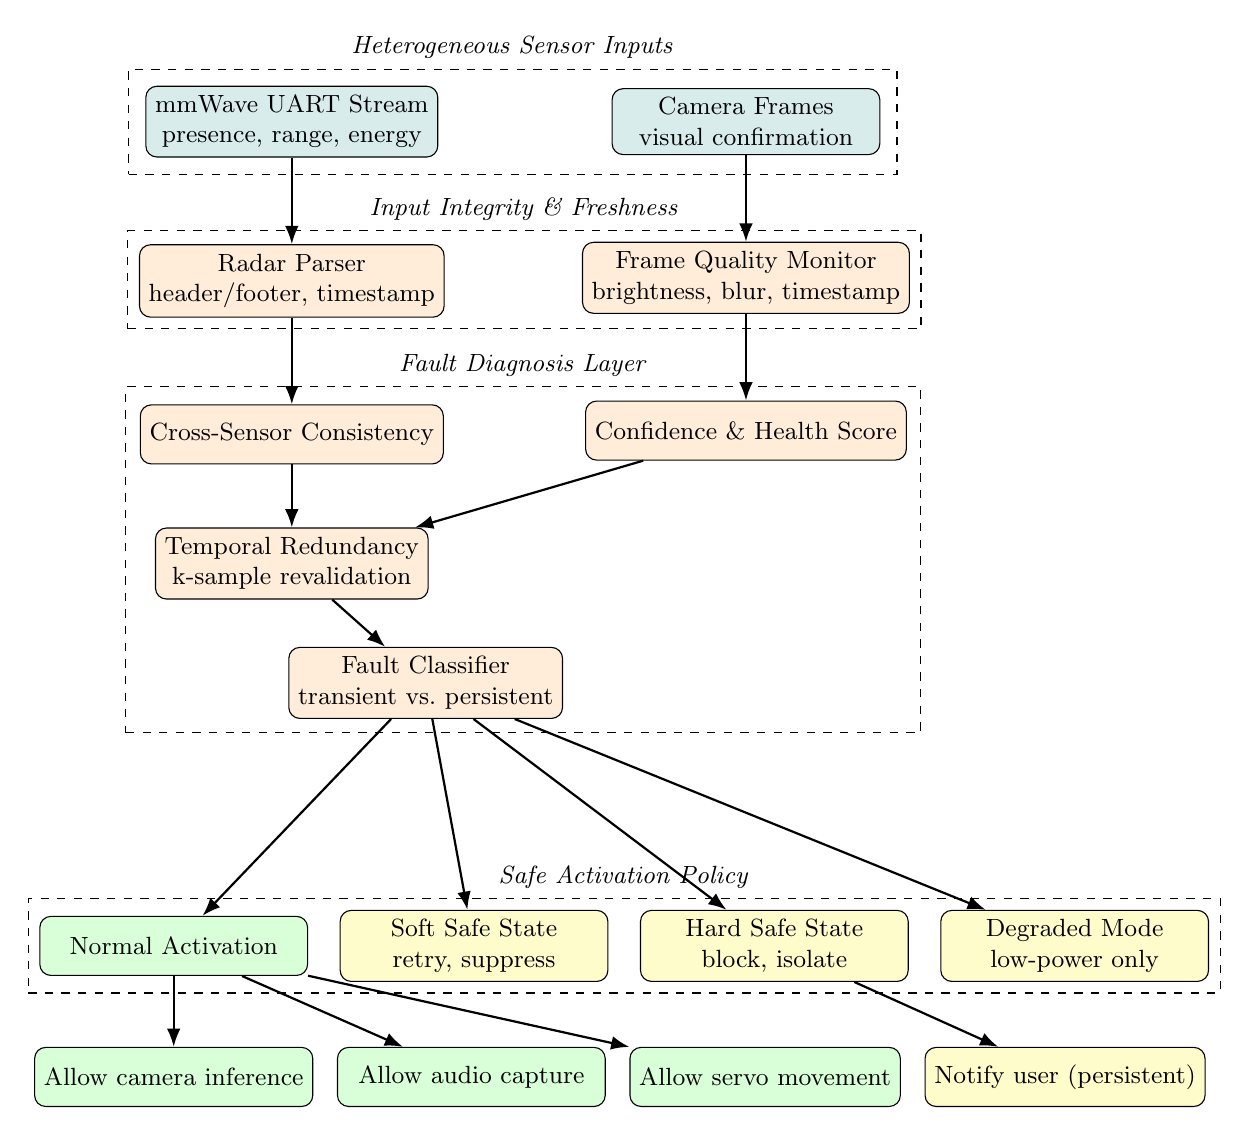
\begin{tikzpicture}[
    node distance=0.9cm and 1.2cm,
    block/.style={draw, rounded corners, align=center, minimum width=3.4cm,
                  minimum height=0.75cm, font=\small},
    sblock/.style={block, fill=teal!15},
    dblock/.style={block, fill=orange!15},
    pblock/.style={block, fill=yellow!20},
    oblock/.style={block, fill=green!15},
    arrow/.style={-Latex, thick}
  ]
    % Sensor inputs
    \node[sblock] (radar) {mmWave UART Stream\\presence, range, energy};
    \node[sblock, right=2.2cm of radar] (cam) {Camera Frames\\visual confirmation};
    \node[draw, dashed, fit=(radar)(cam), inner sep=6pt, label=above:{\small\textit{Heterogeneous Sensor Inputs}}] (inputs) {};

    % Integrity layer
    \node[dblock, below=1.1cm of radar] (rparser) {Radar Parser\\header/footer, timestamp};
    \node[dblock, below=1.1cm of cam] (fqm) {Frame Quality Monitor\\brightness, blur, timestamp};
    \node[draw, dashed, fit=(rparser)(fqm), inner sep=4pt, label=above:{\small\textit{Input Integrity \& Freshness}}] (integ) {};

    % Fault diagnosis
    \node[dblock, below=1.1cm of rparser] (csc) {Cross-Sensor Consistency};
    \node[dblock, below=1.1cm of fqm] (hs) {Confidence \& Health Score};
    \node[dblock, below=0.8cm of csc] (tr) {Temporal Redundancy\\k-sample revalidation};
    \node[dblock, below=0.6cm of tr, xshift=1.7cm] (fc) {Fault Classifier\\transient vs.\ persistent};
    \node[draw, dashed, fit=(csc)(hs)(tr)(fc), inner sep=5pt, label=above:{\small\textit{Fault Diagnosis Layer}}] (diag) {};

    % Activation policy
    \node[oblock, below=2.5cm of fc, xshift=-3.2cm] (na) {Normal Activation};
    \node[pblock, right=0.4cm of na] (ss) {Soft Safe State\\retry, suppress};
    \node[pblock, right=0.4cm of ss] (hs2) {Hard Safe State\\block, isolate};
    \node[pblock, right=0.4cm of hs2] (deg) {Degraded Mode\\low-power only};
    \node[draw, dashed, fit=(na)(ss)(hs2)(deg), inner sep=4pt, label=above:{\small\textit{Safe Activation Policy}}] (policy) {};

    % Outputs
    \node[oblock, below=0.9cm of na] (o1) {Allow camera inference};
    \node[oblock, right=0.3cm of o1] (o2) {Allow audio capture};
    \node[oblock, right=0.3cm of o2] (o3) {Allow servo movement};
    \node[pblock, right=0.3cm of o3] (o4) {Notify user (persistent)};

    % Arrows
    \draw[arrow] (radar) -- (rparser);
    \draw[arrow] (cam) -- (fqm);
    \draw[arrow] (rparser) -- (csc);
    \draw[arrow] (fqm) -- (hs);
    \draw[arrow] (csc) -- (tr);
    \draw[arrow] (hs) -- (tr);
    \draw[arrow] (tr) -- (fc);
    \draw[arrow] (fc) -- (na);
    \draw[arrow] (fc) -- (ss);
    \draw[arrow] (fc) -- (hs2);
    \draw[arrow] (fc) -- (deg);
    \draw[arrow] (na) -- (o1);
    \draw[arrow] (na) -- (o2);
    \draw[arrow] (na) -- (o3);
    \draw[arrow] (hs2) -- (o4);
  \end{tikzpicture}
  \caption{Proposed fault-tolerant activation subsystem architecture.}
  \label{fig:arch}
\end{figure}

\subsection{Architecture Blocks}

\subsubsection{Radar Input Path}

The mmWave sensor communicates over UART at 3.3~V logic.
The \textbf{Radar Parser} processes each incoming frame:
\begin{itemize}
  \item Validates frame header and footer bytes (integrity check).
  \item Timestamps the frame on arrival (\texttt{esp\_timer\_get\_time()}).
  \item Extracts range-gate energy and presence state.
  \item Marks the frame stale if it arrives after a configurable deadline.
\end{itemize}

A packet-drop counter tracks consecutive missing frames.
After $N_{\text{drop}}$ consecutive drops, the parser flags a UART transport fault.

\subsubsection{Camera Input Path}

The \textbf{Frame Quality Monitor} validates each captured frame:
\begin{itemize}
  \item \textbf{Timestamp check:} frame age $>$ $T_{\text{stale}}$ (e.g., 250~ms)
        flags a timing fault.
  \item \textbf{Brightness gate:} mean pixel luminance below $L_{\min}$ flags a
        low-light degradation.
  \item \textbf{Blur estimate:} variance of a Laplacian edge filter below
        $\sigma^2_{\min}$ flags motion blur.
\end{itemize}

Frame quality scores feed into the per-sensor confidence score $C_i$
(Equation~\ref{eq:confidence}).

\subsubsection{Fault Diagnosis Layer}

The diagnosis layer performs three operations in sequence each decision window:
\begin{enumerate}
  \item \textbf{Cross-sensor consistency check.}
        If radar reports presence and camera reports no user (or vice versa),
        an inconsistency flag is raised.
        The diagnosis layer does not immediately decide which sensor is correct.
  \item \textbf{Confidence and health scoring.}
        Each sensor is assigned a score $C_i \in [0, 1]$ using
        Equation~\ref{eq:confidence}.
        Weights $w_s$, $w_f$, $w_t$ are tunable; a default configuration is
        $w_s = 0.5$, $w_f = 0.3$, $w_t = 0.2$.
  \item \textbf{Temporal redundancy.}
        A sliding window of $k$ consecutive decision samples is maintained.
        A fault is classified as \emph{transient} if inconsistency occurred in fewer
        than $k_{\text{hard}}$ of the last $k$ samples, and \emph{persistent} if
        inconsistency has lasted for $k_{\text{hard}}$ or more consecutive windows.
\end{enumerate}

\subsubsection{Fault Classifier}

The fault classifier maps the diagnosis output to a policy state:
\begin{itemize}
  \item \textbf{No inconsistency, high confidence} $\to$ Normal Activation.
  \item \textbf{Inconsistency, transient} $\to$ Soft Safe State.
  \item \textbf{Inconsistency, persistent} $\to$ Hard Safe State.
  \item \textbf{Both sensors degraded or faulted} $\to$ Degraded Mode.
\end{itemize}

\subsection{ESP32-S3 FreeRTOS Task Model}

The subsystem maps onto four FreeRTOS tasks:

\begin{table}[H]
\centering
\caption{FreeRTOS task allocation.}
\label{tab:tasks}
\small
\begin{tabular}{llll}
\toprule
\textbf{Task} & \textbf{Core} & \textbf{Priority} & \textbf{Function}\\
\midrule
\texttt{radar\_rx\_task}     & Core 0 & High   & UART receive, parser, freshness stamp\\
\texttt{camera\_task}        & Core 1 & High   & Frame capture, format, quality check\\
\texttt{diagnosis\_task}     & Core 0 & Medium & Consistency check, scoring, classification\\
\texttt{activation\_gk\_task}& Core 0 & Medium & Policy enforcement, output gating\\
\bottomrule
\end{tabular}
\end{table}

The \textbf{Task Watchdog Timer (TWDT)} monitors \texttt{radar\_rx\_task} and
\texttt{camera\_task} for stalls~\cite{espressif_watchdog}.
A stalled task that does not call \texttt{esp\_task\_wdt\_reset()} within the watchdog
period (configured at 5~s) triggers a watchdog event, logged as a timing fault and
escalating the diagnosis state.

%=================================================================
\section{Fault Model and Diagnosis Logic}
\label{sec:faultmodel}

\subsection{Fault Taxonomy}

Following Avizienis et al.~\cite{avizienis2004}, faults in this subsystem are
classified along four axes: source, nature, duration, and detectability.

\subsubsection{By Source}

\begin{description}
  \item[Sensing faults.] Originate in the physical transducer or its immediate
    interface: radar clutter, camera low-light, radar multipath reflection.
  \item[Communication faults.] Originate in data transport: UART packet drops,
    PSRAM bus contention, camera DMA buffer overrun.
  \item[Timing faults.] Originate in task scheduling or resource contention: stale
    frames, over-long inference windows delaying the diagnosis task, watchdog events.
  \item[Environmental faults.] Originate outside the sensor: fan, moving curtain,
    reflective surface, sudden lighting change.
\end{description}

\subsubsection{By Duration}

\begin{description}
  \item[Transient faults.] Last one or a few decision windows; may self-resolve.
    Examples: brief radar glitch from a passing vehicle, single dropped UART packet.
  \item[Persistent faults.] Persist across $k_{\text{hard}}$ consecutive windows.
    Examples: camera initialization failure, misaligned radar installation.
\end{description}

\subsubsection{SDC-Like (Silent Data Corruption) Faults}

A particularly dangerous sub-class is outputs that appear valid but conflict with
system state.
Example: the radar timestamp is fresh and the presence bit is set, but the camera has
been dark for 10~seconds, and room-level ambient sensors suggest no occupancy.
These faults are addressed by invariant checks: if presence is asserted for longer
than $T_{\text{max\_present}}$ without any camera visual confirmation event, a
fault is flagged.

\subsection{Fault Detection Rules}

\begin{table}[H]
\centering
\caption{Fault detection rules and response actions.}
\label{tab:faultmodel}
\small
\begin{tabular}{p{2.8cm}p{2.6cm}p{3.0cm}p{3.4cm}}
\toprule
\textbf{Fault Class} & \textbf{Example} & \textbf{Observable Symptom} & \textbf{Response}\\
\midrule
Camera false negative & Low light or occlusion & Radar present; camera absent & Revalidate; soft safe state\\
Radar false positive & Fan/curtain/reflection & Radar present; camera no user & Delay activation; request confirmation\\
UART/transport fault & Dropped radar packet & Missing/stale radar timestamp & Parser reset; suppress activation\\
Timing fault & Camera task delay & Fusion uses stale frame & Reject frame; watchdog recovery\\
Persistent sensor fault & Camera init failure & Repeated visual failure & Hard safe state; isolate camera\\
SDC-like output & Stale plausible data & Valid-looking data conflicts with state & Invariant check; rollback health state\\
\bottomrule
\end{tabular}
\end{table}

\subsection{Diagnosis Decision Flow}

Figure~\ref{fig:diagnosis} shows the logic applied each decision window.

\begin{figure}[H]
  \centering
  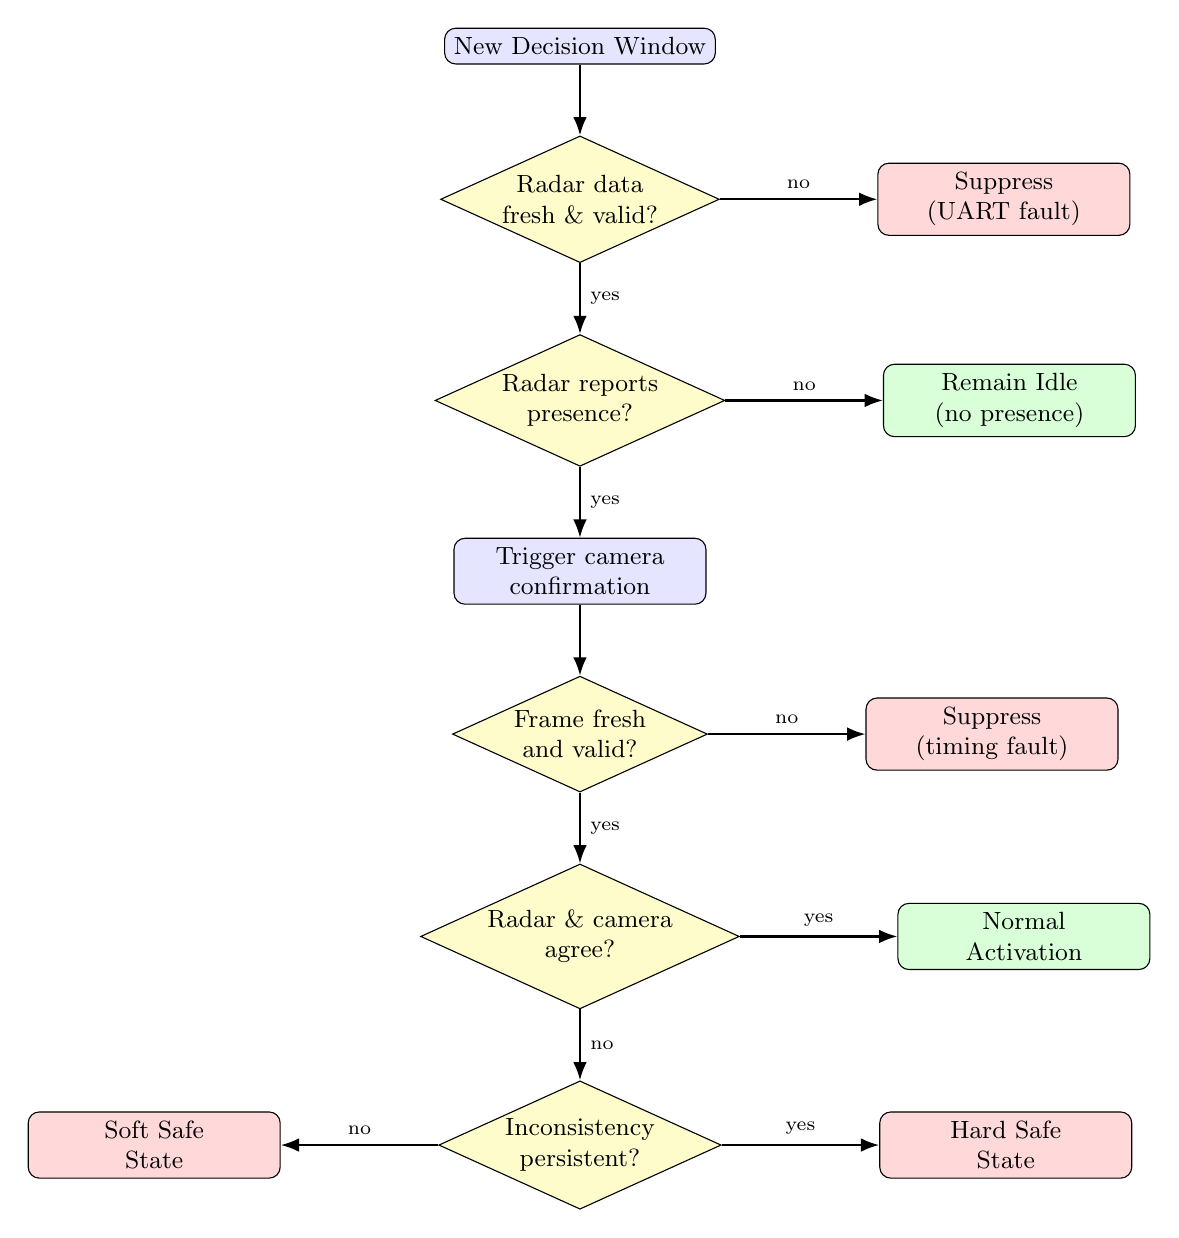
\begin{tikzpicture}[
    node distance=0.9cm,
    decision/.style={diamond, draw, align=center, font=\small, aspect=2.2,
                     inner sep=1pt, fill=yellow!20},
    process/.style={rectangle, draw, rounded corners, align=center, font=\small,
                    minimum width=3.2cm, fill=blue!10},
    safe/.style={rectangle, draw, rounded corners, align=center, font=\small,
                 minimum width=3.2cm, fill=red!15},
    ok/.style={rectangle, draw, rounded corners, align=center, font=\small,
               minimum width=3.2cm, fill=green!15},
    arrow/.style={-Latex, thick}
  ]
    \node[process] (start) {New Decision Window};
    \node[decision, below=of start] (radarfresh) {Radar data\\fresh \& valid?};
    \node[safe, right=2.0cm of radarfresh] (suprad) {Suppress\\(UART fault)};
    \node[decision, below=of radarfresh] (radpresent) {Radar reports\\presence?};
    \node[ok, right=2.0cm of radpresent] (idle) {Remain Idle\\(no presence)};
    \node[process, below=of radpresent] (camtrig) {Trigger camera\\confirmation};
    \node[decision, below=of camtrig] (framefresh) {Frame fresh\\and valid?};
    \node[safe, right=2.0cm of framefresh] (supcam) {Suppress\\(timing fault)};
    \node[decision, below=of framefresh] (agree) {Radar \& camera\\agree?};
    \node[ok, right=2.0cm of agree] (normal) {Normal\\Activation};
    \node[decision, below=of agree] (persist) {Inconsistency\\persistent?};
    \node[safe, right=2.0cm of persist] (hard) {Hard Safe\\State};
    \node[safe, left=2.0cm of persist] (soft) {Soft Safe\\State};

    \draw[arrow] (start) -- (radarfresh);
    \draw[arrow] (radarfresh) -- node[right,font=\scriptsize]{yes} (radpresent);
    \draw[arrow] (radarfresh) -- node[above,font=\scriptsize]{no} (suprad);
    \draw[arrow] (radpresent) -- node[right,font=\scriptsize]{yes} (camtrig);
    \draw[arrow] (radpresent) -- node[above,font=\scriptsize]{no} (idle);
    \draw[arrow] (camtrig) -- (framefresh);
    \draw[arrow] (framefresh) -- node[right,font=\scriptsize]{yes} (agree);
    \draw[arrow] (framefresh) -- node[above,font=\scriptsize]{no} (supcam);
    \draw[arrow] (agree) -- node[above,font=\scriptsize]{yes} (normal);
    \draw[arrow] (agree) -- node[right,font=\scriptsize]{no} (persist);
    \draw[arrow] (persist) -- node[above,font=\scriptsize]{yes} (hard);
    \draw[arrow] (persist) -- node[above,font=\scriptsize]{no} (soft);
  \end{tikzpicture}
  \caption{Diagnosis decision logic per activation window.}
  \label{fig:diagnosis}
\end{figure}

%=================================================================
\section{Safe-State and Recovery Policy}
\label{sec:safestate}

\subsection{State Machine Overview}

The activation subsystem is modeled as a state machine over seven states.
Figure~\ref{fig:statemachine} illustrates the transitions.

\begin{figure}[H]
  \centering
  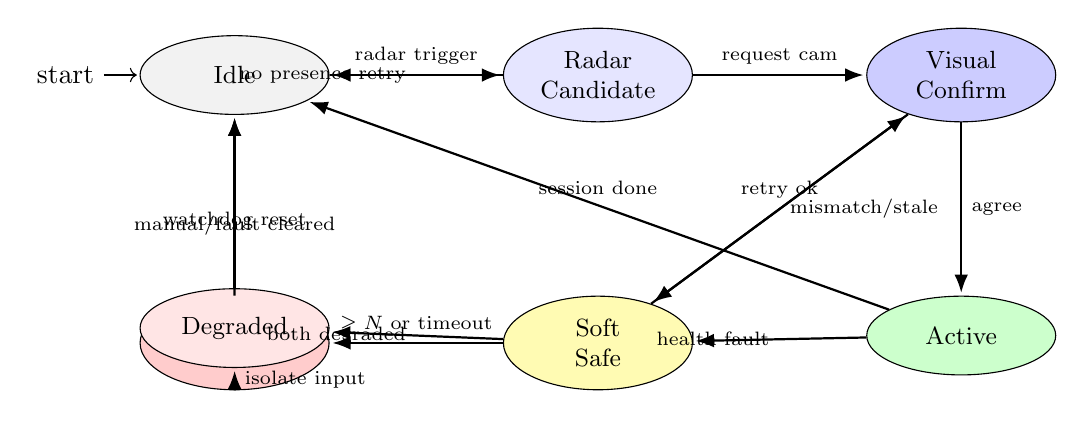
\begin{tikzpicture}[
    shorten >=1pt,
    node distance=2.2cm,
    state/.style={draw, ellipse, align=center, font=\small,
                  minimum width=2.4cm, minimum height=1.0cm},
    arrow/.style={-Latex, thick, font=\scriptsize},
    auto
  ]
    \node[state, initial, fill=gray!10] (idle) {Idle};
    \node[state, fill=blue!10, right=of idle] (rc)   {Radar\\Candidate};
    \node[state, fill=blue!20, right=of rc]   (vc)   {Visual\\Confirm};
    \node[state, fill=green!20, below=of vc]  (act)  {Active};
    \node[state, fill=yellow!30, below=of rc] (ss)   {Soft\\Safe};
    \node[state, fill=red!20, left=of ss]     (hs)   {Hard\\Safe};
    \node[state, fill=red!10, below=of idle]  (deg)  {Degraded};

    \draw[arrow] (idle) -- node[above]{radar trigger} (rc);
    \draw[arrow] (rc)   -- node[above]{request cam} (vc);
    \draw[arrow] (vc)   -- node[right]{agree} (act);
    \draw[arrow] (act)  -- node[above]{session done} (idle);
    \draw[arrow] (vc)   -- node[right]{mismatch/stale} (ss);
    \draw[arrow] (rc)   -- node[left]{no presence retry} (idle);
    \draw[arrow] (ss)   -- node[above]{retry ok} (vc);
    \draw[arrow] (ss)   -- node[above]{$\geq N$ or timeout} (hs);
    \draw[arrow] (hs)   -- node[below]{manual/fault cleared} (idle);
    \draw[arrow] (act)  -- node[left]{health fault} (ss);
    \draw[arrow] (ss)   -- node[left]{both degraded} (deg);
    \draw[arrow] (hs)   -- node[right]{isolate input} (deg);
    \draw[arrow] (deg)  -- node[below]{watchdog reset} (idle);
  \end{tikzpicture}
  \caption{Activation state machine. Safe states (yellow/red) suppress activation.}
  \label{fig:statemachine}
\end{figure}

\subsection{Soft Safe State}

The soft safe state is entered when a \textbf{transient inconsistency} is detected.

\begin{itemize}
  \item Full activation (camera inference, audio, actuation) is \textbf{suppressed}.
  \item The system collects another radar sample and camera frame.
  \item Timestamps and health scores are re-evaluated.
  \item If consistency is restored within the bounded time window $T_{\text{retry}}$,
        the system transitions back to VisualConfirm.
  \item If inconsistency persists beyond $T_{\text{retry}}$ or repeats $N$ times,
        the system escalates to Hard Safe State.
\end{itemize}

\subsection{Hard Safe State}

The hard safe state is entered when a \textbf{persistent inconsistency} is detected.

\begin{itemize}
  \item Automatic activation is \textbf{blocked completely}.
  \item The low-confidence or faulted sensor input is \textbf{isolated} from the
        fusion computation.
  \item The system optionally notifies the user (e.g., OLED message or audio tone)
        that reduced sensing is in effect.
  \item Minimal power operation is maintained (radar sentinel continues; camera is
        paused).
  \item Exit requires either manual reset or watchdog-supervised sensor re-initialization.
\end{itemize}

\subsection{Recovery Block for Visual Confirmation}

A classical \textbf{recovery block}~\cite{randell1975} is applied to the visual
confirmation step:

\begin{enumerate}
  \item \textbf{Primary confirmer:} face/body detector (ESP-DL HumanFaceDetect INT8).
        Acceptance test: confidence score $> \tau_{\text{face}}$ and bounding box
        within valid range.
  \item \textbf{Alternate confirmer:} frame-difference motion detector.
        If the primary confirmer fails or times out, fall back to whether significant
        pixel-delta motion is detected in the expected detection zone.
  \item \textbf{Acceptance test for alternate:} motion delta $> \delta_{\min}$ in
        the center region.
  \item \textbf{Recovery failure:} if alternate also fails acceptance, the system
        remains in Soft Safe State and decrements the retry counter.
\end{enumerate}

This matches the recovery-block design philosophy:
\emph{try the primary method; if its output passes the acceptance test, proceed;
otherwise try the alternate; if the alternate also fails, enter safe state.}

\subsection{Confidence Score Fusion}

The per-sensor confidence score from Equation~\ref{eq:confidence} is computed as
follows for each decision window:

\begin{align}
  S_i &= \begin{cases}1.0 & \text{sensors agree on presence/absence}\\0.0 & \text{disagreement}\end{cases}\\
  F_i &= \max\!\left(0,\; 1 - \frac{t_{\text{now}} - t_{\text{sample}}}{T_{\text{stale}}}\right)\\
  T_i &= \begin{cases}1.0 & \text{TWDT not triggered, no queue overflow}\\0.0 & \text{watchdog or overflow detected}\end{cases}
\end{align}

If $C_i < \tau_C$ (threshold, e.g., 0.6), the system suppresses activation regardless
of the binary presence decision.

%=================================================================
\section{Evaluation Plan and Metrics}
\label{sec:eval}

\subsection{Evaluation Design}

Four activation controllers are compared:
\begin{enumerate}
  \item \textbf{Radar-only baseline.} Activate on any radar presence signal.
  \item \textbf{Camera-only baseline.} Activate on any face-detected frame.
  \item \textbf{Naive AND/OR fusion.} Activate on AND (strict) or OR (permissive)
        of both sensor outputs; no fault diagnosis.
  \item \textbf{Proposed fault-tolerant fusion.} Confidence scoring, cross-sensor
        diagnosis, transient/persistent classification, soft/hard safe states.
\end{enumerate}

\subsection{Fault Injection Tests}

Following Moradi and Denil~\cite{moradi2020faultinj}, faults are injected at the
software level by intercepting sensor data before it reaches the diagnosis layer:

\begin{table}[H]
\centering
\caption{Fault injection test cases.}
\label{tab:faultinj}
\small
\begin{tabular}{p{3.5cm}p{4.5cm}p{4.5cm}}
\toprule
\textbf{Fault Type} & \textbf{Injection Method} & \textbf{Target Metric}\\
\midrule
Radar packet drops     & Drop 1-in-$N$ UART frames randomly & FAR, MDR, fault coverage\\
Radar framing error    & Corrupt header/footer bytes & Fault coverage, detection latency\\
Camera frame blackout  & Replace frame with all-zero buffer & MDR, soft safe state rate\\
Camera motion blur     & Convolve with Gaussian kernel & Fault coverage\\
Stale camera frame     & Freeze timestamp for 500~ms & Timing fault detection rate\\
Induced task delay     & Insert \texttt{vTaskDelay} in camera task & TWDT trigger rate\\
Low-light degradation  & Scale frame luminance to 20\% & Camera health score, MDR\\
UART transport silence & Block UART RX for 2~s & Hard safe state transition time\\
\bottomrule
\end{tabular}
\end{table}

\subsection{Environmental Stress Tests}

Real-environment tests are conducted in the target room with the physical hardware:

\begin{itemize}
  \item Empty room (no occupant): tests false activation rate.
  \item Single user entering and exiting the detection zone.
  \item Static seated user: tests stationary detection.
  \item Low-light condition (lights off): tests camera degradation handling.
  \item Reflective surface (mirror placed in radar field): tests radar clutter.
  \item Moving fan: tests nuisance motion rejection.
\end{itemize}

\subsection{Metrics}

\begin{align}
  \text{FAR} &= \frac{\text{False Activations}}{\text{Total Non-user Trials}}
  \label{eq:far}\\[4pt]
  \text{MDR} &= \frac{\text{Missed Activations}}{\text{Total Valid User Trials}}
  \label{eq:mdr}\\[4pt]
  \text{Fault Coverage} &= \frac{\text{Detected Injected Faults}}{\text{Total Injected Faults}}
  \label{eq:fc}
\end{align}

Additional metrics:
\begin{itemize}
  \item \textbf{Detection latency:} time from fault injection to fault flag.
  \item \textbf{Time-to-safe-state:} time from fault detection to safe-state entry.
  \item \textbf{Recovery time:} time from fault clearance to Normal Activation.
  \item \textbf{Camera duty cycle:} fraction of time camera is actively capturing
        (proxy for energy and privacy exposure).
  \item \textbf{Activation latency overhead:} added delay of fault-tolerant fusion
        relative to the naive baseline.
\end{itemize}

\subsection{Expected Results}

The proposed system is expected to:
\begin{itemize}
  \item Reduce FAR relative to radar-only (which has no semantic check).
  \item Reduce MDR relative to strict AND fusion (which fails if either sensor has
        a transient fault).
  \item Achieve higher fault coverage than naive fusion (which does not diagnose
        disagreements).
  \item Incur moderate activation latency overhead ($<$500~ms) due to revalidation.
\end{itemize}

The primary tradeoff is slightly higher \textbf{activation latency} because the
soft-safe-state revalidation loop adds bounded delay before allowing activation.
This tradeoff is acceptable for an assistive system where false activations carry
privacy costs.

%=================================================================
\section{Analysis of Existing Solutions vs.\ Proposed Improvement}
\label{sec:analysis}

Table~\ref{tab:comparison} compares all known approaches against the proposed system
on six fault-tolerance dimensions.

\begin{table}[H]
\centering
\caption{Comparison of known approaches and proposed improvement.}
\label{tab:comparison}
\small
\begin{tabularx}{\textwidth}{lXXXX}
\toprule
\textbf{Dimension} & \textbf{Radar-only} & \textbf{Camera-only} & \textbf{Naive Fusion} & \textbf{Proposed}\\
\midrule
Heterogeneous redundancy &
  No &
  No &
  Yes (implicit) &
  \textbf{Yes (explicit)}\\
Cross-sensor diagnosis &
  No &
  No &
  No &
  \textbf{Yes}\\
Transient/persistent classification &
  No &
  No &
  No &
  \textbf{Yes}\\
Soft/hard safe states &
  No &
  No &
  No &
  \textbf{Yes}\\
Confidence/freshness scoring &
  No &
  No &
  No &
  \textbf{Yes}\\
Fault-injection evaluation &
  No &
  No &
  No &
  \textbf{Yes}\\
Timing fault detection (TWDT) &
  No &
  No &
  No &
  \textbf{Yes}\\
Recovery block for vision &
  No &
  No &
  No &
  \textbf{Yes}\\
\bottomrule
\end{tabularx}
\end{table}

The gaps in existing approaches translate directly to failure modes:
\begin{itemize}
  \item \textbf{Radar-only gap:} no independent validation means radar clutter
        directly causes false activation with no recourse.
  \item \textbf{Camera-only gap:} high resource consumption and environmental
        sensitivity create excessive missed activations in low-light conditions.
  \item \textbf{Naive fusion gap:} AND logic causes MDR to increase whenever one
        sensor experiences a transient fault; OR logic causes FAR to increase when
        either sensor is noisy.
        Neither diagnoses the disagreement.
\end{itemize}

The proposed health-aware activation controller addresses all three gaps without
requiring a GPU or deep-learning pipeline.

%=================================================================
\section{Expected Contribution and Limitations}
\label{sec:contribution}

\subsection{Expected Contributions}

\begin{enumerate}
  \item \textbf{Reduced false activation rate} relative to radar-only activation,
        because the camera provides semantic rejection of clutter.
  \item \textbf{Reduced missed activation rate} relative to strict naive AND fusion,
        because transient faults enter a soft safe state and retry rather than
        blocking immediately.
  \item \textbf{Reduced privacy and energy exposure} relative to camera-heavy
        activation, because the camera is activated on-demand only after radar trigger,
        and suppressed during faults.
  \item \textbf{Explicit fault coverage} measured by fault injection, providing a
        quantified dependability characterization rather than only a nominal accuracy
        number.
  \item \textbf{Demonstration of classical fault-tolerance principles}---redundancy,
        error detection, diagnosis, recovery blocks, and graceful degradation---applied
        to a modern ESP32-S3 edge AI activation pipeline.
\end{enumerate}

\subsection{Why This Matters}

For a privacy-preserving assistive platform, ambiguity should not automatically trigger
camera, audio, or actuator activation.
The system should explicitly represent uncertainty and enter a safe state until
confidence improves.
This is the correct fault-tolerant design stance for a system where false activation
carries privacy costs and missed activation carries assistance costs.

\subsection{Limitations}

\begin{itemize}
  \item The project uses a low-cost 24~GHz UART-output mmWave module, not a
        research-grade radar with raw radar cubes.
        Advanced radar OOD algorithms such as HOOD~\cite{kahya2025hood} require
        richer radar data (Doppler profiles, range-Doppler maps) and are used here
        as conceptual motivation rather than directly reproduced.
  \item The evaluation is room-scale and involves limited occupancy scenarios and
        limited environmental variation.
        Generalization to multi-room, multi-occupant, or outdoor settings is not
        evaluated.
  \item The activation latency overhead from soft-safe-state revalidation is bounded
        but nonzero.
        For applications requiring sub-100~ms activation latency, this tradeoff would
        need re-evaluation.
  \item The confidence weights $w_s$, $w_f$, $w_t$ and thresholds $\tau_C$,
        $k_{\text{hard}}$, $T_{\text{stale}}$ are tuned empirically in the target
        environment.
        Automatic threshold adaptation is left for future work.
\end{itemize}

%=================================================================
\section{Conclusion}
\label{sec:conclusion}

This report has presented a fault-tolerant activation subsystem for a room-scale
assistive sensing platform built on the ESP32-S3.
The system addresses a problem that is distinct from pure sensing: making the
activation decision dependable under realistic embedded faults, not merely optimizing
detection accuracy under nominal conditions.

The proposed architecture uses:
\begin{itemize}
  \item \textbf{Heterogeneous redundancy} (radar + camera) to cover the failure modes
        of each individual modality.
  \item \textbf{Cross-sensor consistency checking} to detect disagreements without
        immediately committing to either sensor's output.
  \item \textbf{Temporal redundancy} (k-sample revalidation) to distinguish transient
        from persistent faults.
  \item \textbf{Confidence and freshness scoring} to weight sensor inputs by their
        current reliability.
  \item \textbf{Soft and hard safe states} to implement fail-safe behavior at two
        levels of fault severity.
  \item \textbf{Recovery blocks} for the visual confirmation step.
  \item \textbf{Watchdog-based timing fault detection} using the ESP-IDF TWDT.
  \item \textbf{Fault-injection evaluation} to characterize dependability beyond
        nominal accuracy.
\end{itemize}

These are classical fault-tolerance principles applied to a modern, constrained,
embedded edge AI system.
The contribution is not a new sensing algorithm, but a new architectural pattern for
making sensing-based activation decisions trustworthy.

For privacy-preserving assistive systems, this trustworthiness is not optional---it
is a core requirement.
A system that can activate itself incorrectly, or that silently fails to activate,
violates the user's autonomy, privacy, and ability to rely on the assistant.
The fault-tolerant activation boundary proposed here is a step toward embedded edge AI
systems that are not only capable but also dependable.

%=================================================================
\begin{thebibliography}{99}

\bibitem{avizienis2004}
A.~Avizienis, J.-C.~Laprie, B.~Randell, and C.~Landwehr,
``Basic Concepts and Taxonomy of Dependable and Secure Computing,''
\textit{IEEE Transactions on Dependable and Secure Computing},
vol.~1, no.~1, pp.~11--33, Jan.--Mar.\ 2004.

\bibitem{li2023mmwave}
S.~Li and R.~Hishiyama,
``An Indoor People Counting and Tracking System Using mmWave Sensor and Sub-sensors,''
\textit{IFAC-PapersOnLine},
2023, doi:~10.1016/j.ifacol.2023.10.577.

\bibitem{yu2026mscaf}
Y.~Yu, H.~R.~Karimi, L.~Gelman, J.~Tian, and P.~Mei,
``A Novel Multi-Source Sensor Correlation Adaptive Fusion Framework with Uncertainty
Quantification for Intelligent Fault Diagnosis,''
\textit{Reliability Engineering \& System Safety},
vol.~267, 2026, Art.\ no.~111812, doi:~10.1016/j.ress.2025.111812.

\bibitem{moradi2020faultinj}
M.~Moradi and J.~Denil,
``Machine-Learning Assisted Model-Implemented Fault Injection,''
\textit{CEUR Workshop Proceedings},
2020.

\bibitem{kahya2025hood}
S.~M.~Kahya, M.~S.~Yavuz, and E.~Steinbach,
``HOOD: Real-Time Human Presence and Out-of-Distribution Detection Using FMCW Radar,''
\textit{IEEE Transactions on Radar Systems},
2025, doi:~10.1109/TRS.2024.3514840.

\bibitem{zhang2026robust}
N.~Zhang, H.~Li, A.~Zahid, Y.~Tian, and W.~Li,
``A Robust mmWave Radar Framework for Accurate People Counting and Motion Classification,''
\textit{Sensors},
vol.~26, no.~4, Art.\ no.~1289, 2026, doi:~10.3390/s26041289.

\bibitem{espressif2023trm}
Espressif Systems,
\textit{ESP32-S3 Series Datasheet and Technical Reference Manual},
2023.
Available: \url{https://www.espressif.com/en/support/documents/technical-documents}

\bibitem{espressif_watchdog}
Espressif Systems,
``Watchdogs,''
\textit{ESP-IDF Programming Guide for ESP32-S3},
2024.
Available: \url{https://docs.espressif.com/projects/esp-idf/en/stable/esp32s3/api-reference/system/wdts.html}

\bibitem{espressif_cam}
Espressif Systems,
\textit{esp32-camera: ESP32 Camera Driver},
GitHub repository.
Available: \url{https://github.com/espressif/esp32-camera}

\bibitem{seeed_mmwave}
Seeed Studio,
``24~GHz mmWave Sensor for XIAO: Human Static Presence,''
2023.
Available: \url{https://wiki.seeedstudio.com/Seeed-Studio-MR24HPC1-mmWave-Human-Static-Presence-Module-Lite/}

\bibitem{randell1975}
B.~Randell,
``System Structure for Software Fault Tolerance,''
\textit{IEEE Transactions on Software Engineering},
vol.~SE-1, no.~2, pp.~220--232, Jun.\ 1975.

\end{thebibliography}

\end{document}
